\begin{frame}
  \frametitle{Emisii continue}
  \begin{itemize}
  \item Probabilitatea emisiilor este modelată cu o lege de distribuție continuă (e.g. normală).
    \begin{equation}
      \label{eq:contin1}
      b_j(o) = \mathcal{N}(o,\mu_j,\sigma_{j}^{2})
    \end{equation}
  \end{itemize}
  \vspace*{1em}
  \begin{center}
    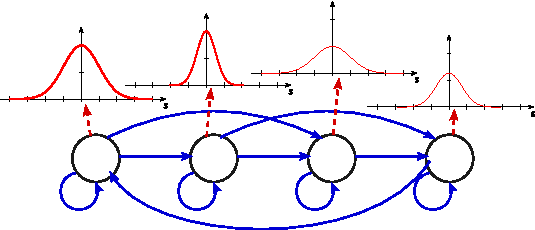
\includegraphics[width=0.9\textwidth]{graphics/other-hmm/continuous.pdf}
  \end{center}
\end{frame}

\begin{frame}
  \frametitle{Mixturi Gaussiene}
  \begin{itemize}
  \item Probabilitatea emisiilor este modelată printr-o mixtură de distribuții normale.
    \begin{equation}
      \label{eq:contin2}
      b_j(o) = \displaystyle\sum_{k=1}^{M} c_{j,k}\mathcal{N}(o,\mu_{j,k},\sigma_{j,k}^2)
    \end{equation}
  \end{itemize}
  \vspace*{1em}
  \begin{center}
    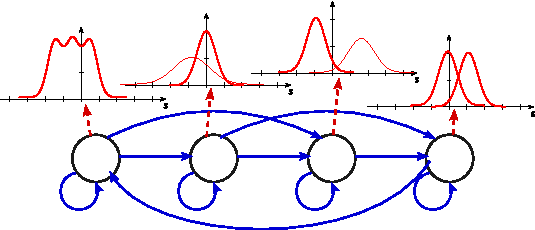
\includegraphics[width=0.9\textwidth]{graphics/other-hmm/mixture.pdf}
  \end{center}
\end{frame}

\begin{frame}
  \frametitle{Modele Markov Ergodice}
  \begin{block}{Modele Markov Ergodice}
    Un lanț Markov se numește \alert{ergodic} dacă din orice stare se poate ajunge în oricare altă stare (nu neaparat într-o singură mutare).\\
    Lanțurile Markov ergodice se mai numesc și \emph{ireductibile}.
  \end{block}
  \vspace*{1em}
  \begin{center}
    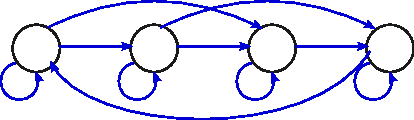
\includegraphics[width=0.8\textwidth]{graphics/other-hmm/ergodic.pdf}
  \end{center}
\end{frame}

\begin{frame}
  \frametitle{Modelul Bakis}
  \begin{block}{Modele Markov Bakis (stânga $\longrightarrow$ dreapta)}
    Un model \alert{Bakis} este unul în care nu este permisă tranziția
    dintr-o stare către o altă stare cu un indice mai mic.
  \end{block}
  \vspace*{1em}
  \begin{center}
    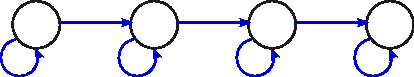
\includegraphics[width=0.8\textwidth]{graphics/other-hmm/left-to-right.pdf}
  \end{center}
\end{frame}